
\marginnote{\href{https://youtu.be/P7a4bjE6Crk}{Video}}
\marginnote{\href{https://ocw.mit.edu/courses/6-041sc-probabilistic-systems-analysis-and-applied-probability-fall-2013/pages/unit-ii/lecture-12/}{Lecture Home}}
\marginnote{\href{https://ocw.mit.edu/courses/6-041sc-probabilistic-systems-analysis-and-applied-probability-fall-2013/e3e0a97e8298a57f911e24c304008870_MIT6_041SCF13_L12.pdf}{Slides}}

Reading: 4.3, 4.5 (no transforms)

This lecture is the end of the core material for the class (probability).

Conditional Expectations: $E[X|Y$
\begin{itemize}
    \item Law of Iterated Expectations
    \item Law of Total Variance
\end{itemize}

\subsection{Conditional Expectations}

\marginpar{1:38)}

\begin{align}
    E[X|Y=y]= \sum_x x p_{X|Y}(x|y)
\end{align}
\myequations{Conditional Expectation}

\begin{align*}
    E[X|Y=y]=\frac{y}{2} \qquad (number)
\end{align*}

\begin{align*}
    E[X|Y=y]=\frac{Y}{2} \qquad (r.v.)
\end{align*}

\marginpar{7:55)}

\begin{align*}
    E[X|Y]=g(Y)\\
    E[X|Y=y]=g(y)\\
    E[E[X|Y]]=E[g(Y)]
\end{align*}

\begin{align}
E[E[X|Y]]=E[X]
\label{eq:law_iter_ex}
\end{align}
\myequations{Law of Iterated Expectation}

\subsection{Law of Total Variance}
\marginpar{15:10)}

\begin{align}
var(X) = E[var(X|Y)] + var(E[X|Y])
\label{eq_law_tot_var}
\end{align}
\myequations{Law of Total Variance}

Proof confusing and no intuition

\subsection{Baby Example}
\marginpar{19:30)}


\subsection{Example}
\marginpar{31m)}

\begin{figure}[ht]
\centering
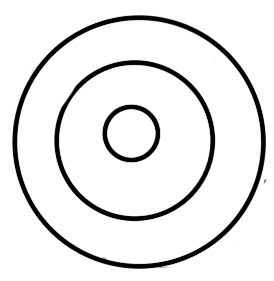
\includegraphics[width=6cm, height=4cm]{images/L11/percent_circle.jpeg}
\caption{x}
\end{figure}

\begin{align*}
var(X) = E[var(X|Y)] + var(E[X|Y]) \qquad (LOTV)
\end{align*}

\begin{align*}
E[X|Y=1] = \frac{1}{2}, \qquad E[X|Y=2] = \frac{3}{2}
\end{align*}

\begin{align*}
var(X|Y=1) = \frac{1}{2}, \qquad var(X|Y=2) = \frac{1}{2}
\end{align*}

\begin{align*}
var(E[X|Y]) = \frac{1}{3} \left(\frac{1}{2} - \frac{7}{6} \right)^2 + \frac{2}{3} \left( \frac{3}{2} - \frac{7}{6} \right)^2
\end{align*}

\subsection{Sum of Random Number of Independent Random Variables}

\marginpar{36m)}

\begin{itemize}
    \item N: \# stores visited
    \item $X_i$: money spent at store i. iid
\end{itemize}


Let $Y=X_1+ \cdots + X_n$

\begin{align*}
    E[Y|N=n] = slides...\\
    = nE[X]
\end{align*}

\subsection{Variance of Sum of Random Number of Independent Random Variables}

\marginpar{44m)}

slide...
EVE:
\begin{align*}
var(Y) = E[var(Y|N)] + var(E[Y|N])\\
 = E[N] var(X) + (E[X])^2 var(N)
\end{align*}